\begin{figure}[tb]
\centering
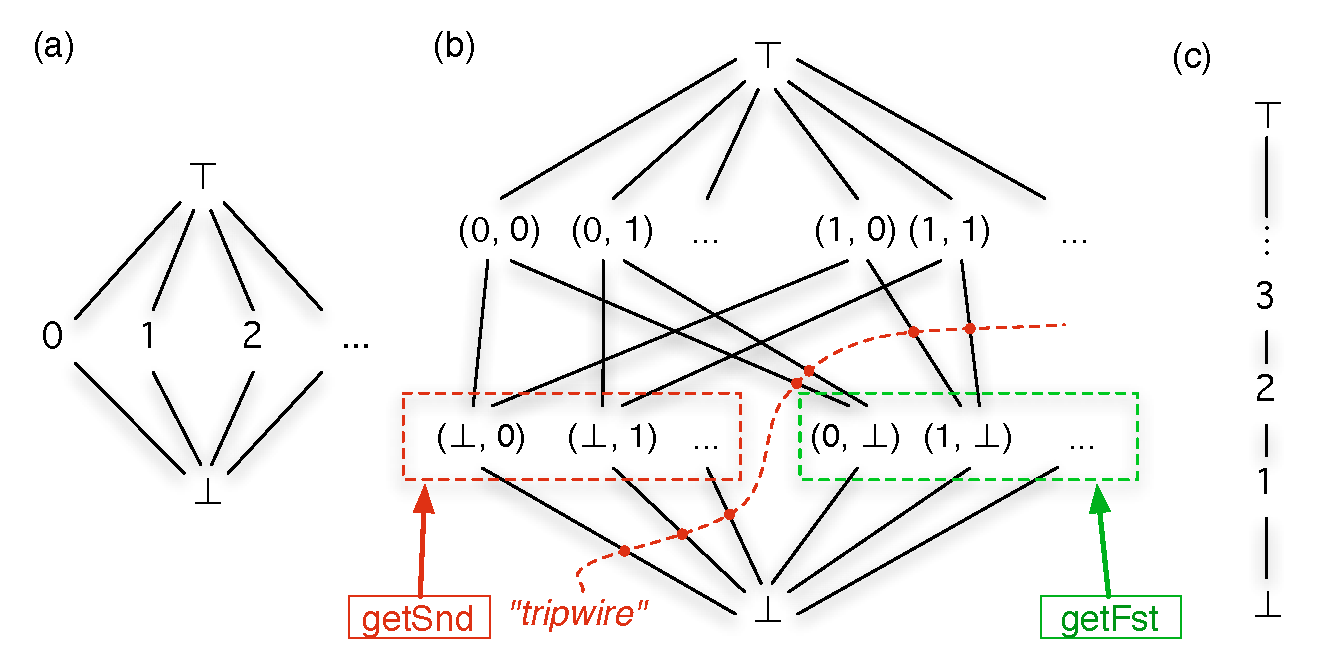
\includegraphics[width=3.3in,natwidth=633px,natheight=319px]{chapter2/figures/ExampleLattices2.pdf} 
  \caption{\footnotesize Example lattices: (a) IVar
    containing a natural number; (b) pair of natural-number-valued IVars; (c)
    positive integers ordered by $\leq$ (see Section~\ref{subsection:bump}).
%    \new{an LVar storing the maximum observation}.  
%    \new{maximum number}.  
    Subfigure (b) is annotated with example threshold
    sets that would correspond to a blocking read of the first or
    second element of the pair (see Sections~\ref{subsection:putget} and \ref{subsection:programming-with-put-and-get}).
    Any state transition crossing the
    ``tripwire'' for \impfnt{getSnd} causes it to unblock
    and return a result.}

  \label{f:lattice-examples}
\end{figure}

\section{Lattices, Stores, and Determinism}\label{section:domains}

As a minimal substrate for LVars, we introduce $\lambdapar$, 
 a parallel call-by-value
$\lambda$-calculus extended with a {\em store} and with communication
primitives $\PUT$ and $\GET$ that operate on data in the store.
The class of programs that we are interested in modeling with
$\lambdapar$ are those with explicit effectful operations on shared
data
structures, in which subcomputations may communicate with each other
via the $\PUT$ and
$\GET$ operations.

In this setting of shared mutable state, the trick
that $\lambdapar$ employs to maintain determinism is that stores
contain {\em LVars}, which are a generalization of
IVars.\footnote{IVars are so named because they are a
    special case of {\em I-structures} \cite{IStructures}---namely,
    those with only one cell.}
Whereas IVars are single-assignment
variables---either empty or filled with an immutable value---an LVar
may have an arbitrary number of states forming a set $D$, which is partially ordered by a relation 
$\myleq$.  An LVar can take on any sequence of states from 
$D$, so long as that sequence respects the partial order---that is,
updates to the LVar (made via the $\PUT$ operation) are
\emph{inflationary} % \emph{monotonic}
 with respect to $\myleq$.  Moreover, the 
 $\GET$ operation allows only limited observations of the LVar's state.  In
this section, we discuss how lattices and stores work in $\lambdapar$
and explain how the semantics of $\PUT$ and $\GET$ together enforce determinism
in $\lambdapar$ programs.

\subsection{Lattices}\label{subsection:domains}

The definition of $\lambdapar$ is parameterized by the choice of $D$: to write concrete $\lambdapar$ programs, one must specify
the set of LVar states that one is interested in working with,
and an ordering on those states.
  Therefore
$\lambdapar$ is actually a \emph{family} of languages, rather than a
single language.

Formally, $D$ is a \emph{bounded} \emph{join-semilattice} augmented
with a greatest element $\top$.  That is, $D$ has the following
structure:
\begin{itemize}
\item $D$ has a least element $\bot$, representing the initial
  ``empty'' state of an LVar.

\item $D$ has a greatest element $\top$, representing the ``error''
  state that results from conflicting updates to an LVar.

\item $D$ comes equipped with a partial order $\myleq$, where $\bot
  \myleq d \myleq \top$ for all $d \in D$.

\item Every pair of elements in $D$ has a least upper bound (lub)
  $\sqcup$.  Intuitively, the existence of a lub for every two
  elements in $D$ means that it is possible for two subcomputations to
  independently update an LVar, and then deterministically merge the
  results by taking the lub of the resulting two states.
\end{itemize}

\noindent Virtually any data structure to which information
is added gradually can be represented as a lattice,
including pairs, arrays, trees, maps, and infinite streams.
%
{In the case of maps or sets, $\sqcup$ could be defined simply as union; for
pointer-based data structures like tries, it could allow for unification of partially-initialized structures.}
%
% , and even atomic counters and reduction variables.  
% \lk{Do people know what``reduction variables'' are?  I don't (although my co-workers seem to, so it's probably fine).}

Figure~\ref{f:lattice-examples} gives three examples of lattices for
common data structures.
% \new{Combinations of different data structures can always be used
%   within the same program simply by unioning their state spaces into
%   one domain $D$.}
The simplest example of a useful lattice is one that
represents the state space of a single-assignment variable (an IVar).
A natural-number-valued IVar, for instance, would correspond to the
lattice in Figure~\ref{f:lattice-examples}(a), that is,
\begin{displaymath}
  D = (\lbrace \top, \bot \rbrace \cup \mathbb{N}, \myleq), 
\end{displaymath}
where the partial order $\myleq$ is defined by setting $\bot \myleq d
\myleq \top$ and $d \myleq d$ for all $d \in D$.  This is a lattice of
height three and infinite width, where the naturals are arranged
horizontally.  After the initial write of some $n \in \mathbb{N}$, any
further conflicting writes would push the state of the IVar to $\top$
(an error).
For instance, if one thread writes $2$ and another writes $1$ to an
IVar (in arbitrary order), the second of the two writes would result
in an error because $2 \sqcup 1 = \top$.

In the lattice of Figure~\ref{f:lattice-examples}(c), on the other
hand, the $\top$ state can never be reached, because the least upper
bound of any two writes is just the maximum of the two.
For instance, if one thread writes $2$ and another writes $1$, the
resulting state will be $2$, since $2 \sqcup 1 = 2$.
Here, the
unreachability of $\top$ models the fact that no conflicting updates
can occur to the LVar.

\subsection{Stores}\label{subsection:stores}

% \amr{A lot of the discussion below can and should be summarized to a simple
%   fact: stores also form a bounded join semilattice. This means that the
%   following: \\
%   ``We use $\top$ as a shorthand for any store that contains a binding to
%   $\top$; for instance, the premise $\lubstore{S_1}{S_2} = \top$ of the {\sc
%     E-ParAppErr} rule says that the lub of $S_1$ and $S_2$ is a
%   store in which some location is bound to $\top$.''  \\
%   would not be quite right. The first occurrence is the top in the store
%   lattice and the second is the top in the D-lattice.\\
%   For clarity it might be necessary to initially define things using $\bot_D$
%   and $\bot_S$ and then say that the subscript will be generally
%   omitted. There is also a slight issue which has to do with the fact that
%   $\bot_S$ is any store that contains any number of locations that are all
%   bound to $\bot$. Similarly to $\topS$. This needs to be made precise. This
%   is all crucial I think because the rest of the paper implicitly assumes
%   that stores do satisfy the axioms of a bounded join-semilattice.}

% \rn{This is definitely a problem for tops.  But is it also a problem
%   for bottoms?  I thought that bottom was simply the empty store, and
%   then performing ``new'' (to add a $l\rightarrow\bot$ binding) does push
%   the state upward.}

% \lk{Now I've gone back to thinking that bottom is the empty store.
%   Need to check with Amr about this, but I've changed the text to
%   reflect that.  Added note to TODO.md.}

% \rn{Regarding the top case... can we mark all the places where we have
%   preconditons like $S = \top$?  Perhaps we can go back and express
%   those as some kind of isError predicate function.  Where isError iff
%   $\top_D \in S$ or $S = \topS$...  I guess we still need $\topS$ if
%   ONLY so that we can sensibly write $\lubstore{S_1}{S_2}$, even
%   though we make sure that state $\topS$ is never reached,
%   transitioning the configuration to {\bf error} instead.}

% \lk{So, the only places where the store can go to $\top$ are in {\sc
%     E-PutValErr} or {\sc E-ParAppErr}, and once either of those steps
%   have been taken we're stuck in $\error$ (technically, we can still
%   take a step, but only to $\error$).  If we just explain this in the
%   text, do we really need to do any more marking of preconditions?}

During the evaluation of a $\lambdapar$ program, a \emph{store} $S$
keeps track of the states of LVars.  Each LVar is represented by a
binding from a location $l$, drawn from a set $\Loc$, to its state,
which is some element $d \in D$.  Although each LVar in a program has
its own state, the states of all the LVars are drawn from the same
lattice $D$.  We can do this with no loss of generality because
lattices corresponding to different types of LVars could always be
unioned into a single lattice (with shared $\top$ and $\bot$
elements).
\new{Alternatively, in a typed formulation of $\lambdapar$, 
  the type of an LVar might determine the lattice of its states.}

\begin{definition}\label{def:store}
A \emph{store} is either a finite partial mapping $S : \Loc \fmap (D-\lbrace \top \rbrace)$, or the distinguished element $\topS$.
\end{definition}

\noindent We use the notation $\extS{S}{l}{d}$ to denote extending $S$
with a binding from $l$ to $d$.  If $l \in \dom{S}$, then
$\extS{S}{l}{d}$ denotes an update to the existing binding for $l$,
rather than an extension.  We can also denote a store by explicitly
writing out all its bindings, using the notation
$\store{\storebinding{l_1}{d_1}, \dots, \storebinding{l_n}{d_n}}$.
%
The state space of stores forms a bounded join-semilattice
augmented with a greatest element, just as
$D$ does, with the empty store $\bot_S$ as its least element and $\topS$ 
as its greatest element.
It is straightforward to lift the $\myleq$ and $\sqcup$ operations defined
on elements of $D$ to the level of stores:

\DefLeqStore

\DefLubStore

\noindent By Definition~\ref{def:store-lub}, if $\lub{d_1}{d_2} =
\top$, then
$\lubstore{\store{\storebinding{l}{d_1}}}{\store{\storebinding{l}{d_2}}}
= \topS$.  
Notice that a store containing a binding $\storebinding{l}{\top}$ can never arise
during the execution of a $\lambdapar$ program, because (as we will
see in Section~\ref{section:programming}) an attempted write that would take
the state of $l$ to $\top$ would raise an error before the write can occur.

\subsection{Communication Primitives}\label{subsection:putget}

% \amr{ I think the properties of the lattice discussed below in the
%   explanation of get should be moved to the subsection that introduces
%   domains. The point is that the structure of domains is motivated by the
%   desire to define good threshold sets. Also I don't understand what it means for
%   a set to be disjoint. Disjoint from what?}

% \lk{``disjoint'' was a mistake; I got rid of it.  I think that we want
%   people to be looking at the {\sc E-GetVal} rule when they read that
%   explanation.  The point of the section is to give some idea of why
%   {\sc E-GetVal} looks so weird.  So I moved it further ahead,
%   instead, to the section where we are starting to talk about the
%   reduction rules.}

The $\NEW$, $\PUT$, and $\GET$ operations create, write to, and read
from LVars, respectively.  The interface is similar to that presented
by mutable references:

\begin{itemize}
\item $\NEW$ extends the store with a binding for a new LVar whose
  initial state is $\bot$, and returns the location $l$ of that LVar
  (\ie, a pointer to the LVar).
\item $\PUT$ takes a pointer to an LVar and a singleton set containing
  a new state and updates the LVar's state to the {\em least upper bound} of the current state and the new state,
  potentially pushing the state of the LVar upward in the
  lattice.  Any update that would take the state of an LVar to $\top$
  results in an error.
\item $\GET$ performs a blocking ``threshold'' read that allows
  limited observations of the state of an LVar.  It takes a pointer to
  an LVar and a \emph{threshold set} $Q$, which is a non-empty subset
  of $D$ that is \emph{pairwise incompatible}, meaning that the lub of
  any two distinct elements in $Q$ is $\top$.  If the LVar's state $d$
  in the lattice is {\em at or above} some $d' \in Q$, the $\GET$
  operation unblocks and returns the singleton set $\lbrace d'
  \rbrace$.  Note that $d'$ is a unique element of $Q$, for if there
  is another $d'' \neq d'$ in the threshold set such that $d'' \myleq
  d$, it would follow that $d' \sqcup d'' \myleq d \neq \top$, which
  contradicts the requirement that $Q$ be pairwise incompatible.
\end{itemize}

\noindent The intuition behind $\GET$ is that
it specifies a subset of the lattice that is ``horizontal'': no two
elements in the threshold set can be above or below one another.  
Intuitively, each element in the threshold set is an
``alarm'' that detects the activation of itself or any state
above it.  One way of visualizing the threshold set for a $\GET$ operation
is as a subset of edges in the lattice that, if crossed, set off the
corresponding alarm.  Together these edges form a ``tripwire''.  This
visualization is pictured in Figure~\ref{f:lattice-examples}(b).  The
threshold set $\stateset{(\bot, 0), (\bot, 1), ...}$ (or a subset thereof)
would pass the incompatibility test, as would the threshold set
$\stateset{(0, \bot), (1, \bot), ...}$ (or a subset thereof), but a
combination of the two would not pass.

\new{Both $\GET$ and $\PUT$ take and return  {\em sets}.  
The fact that $\PUT$ takes a singleton set and $\GET$ returns a
singleton  set (rather than a value $d$) may seem awkward; it
is merely a way to keep the grammar for values simple, and avoid
including set primitives in the language (\eg, for converting $d$ to
$\lbrace d \rbrace$).}

\subsection{Monotonic Store Growth and Determinism}\label{subsection:monotonicity}

In IVar-based languages, a store can only change
in one of two ways: a new binding is added at $\bot$, or a
previously $\bot$ binding is permanently updated to a meaningful value.
It is therefore straightforward in such languages
to define an ordering on stores and establish determinism based on the
fact that stores grow monotonically with respect to the ordering. For
instance, \emph{Featherweight CnC} \cite{CnC}, a single-assignment 
imperative calculus that models the Intel Concurrent Collections (CnC)
system, defines ordering on stores as follows:\footnote{In
  Featherweight CnC, 
  no store location is explicitly bound to $\bot$.
  Instead, if $l \notin \dom{S}$ then $l$ is defined to be at
  $\bot$. %% and locations spring into existence at the time their
  %% permanent values are written.
}

\DefLeqStoreCnC

\noindent 
Our Definition~\ref{def:leqstore} is reminiscent of
Definition~\ref{def:leqstore-cnc}, but Definition~\ref{def:leqstore-cnc}
requires that $S(l)$ and $S'(l)$
be \emph{equal}, instead of our weaker
requirement that $S(l) \myleq S'(l)$ according to the user-provided
partial order $\myleq$.  In $\lambdapar$, stores may grow by updating
existing bindings via repeated $\PUT$s, so
Definition~\ref{def:leqstore-cnc} would be too strong; for instance,
if $\bot \mylt d_1 \myleq d_2$ for distinct $d_1, d_2 \in D$, the relationship
$\leqstore{\store{\storebinding{l}{d_1}}}{\store{\storebinding{l}{d_2}}}$
holds under Definition~\ref{def:leqstore}, but would not hold under
Definition~\ref{def:leqstore-cnc}.  That is, in $\lambdapar$ an LVar
could take on the state $d_1$ followed by $d_2$, which would not be
possible in Featherweight CnC.  We establish in
Section~\ref{section:proof} that $\lambdapar$ remains
deterministic despite the relatively weak $\leqstore{}{}$
relation given in Definition~\ref{def:leqstore}.  The keys to
maintaining determinism are the blocking semantics of the $\GET$
operation and the fact that it allows only \emph{limited} observations
of the state of an LVar.


